\section{照明电路}\label{sec:11-1}

照明电路里的主要设备是电灯。
电灯应该在需要它照明的时候才亮,这就要有个开关(电健)跟它串联,及时通电或断电。
一栋房内的电灯有许多盏,任何一盏的开和关,都不应该影响其他电灯,所以各盏电灯应该并联。

电路中的电流如果过强,导线会过热,设备会损坏,甚至可能引起火灾。
为了避免这种事故,电路中必须有保险装置——保险盒,使电流强度超过规定值时能自动切断电路。
检修电路,更换元件,包括更换保险盒,应该先切断电源,以免触电,这就需要在保险盒前装个总开关。
为了测量用户消耗了多少电能,要在总开关前面装个电度表。连接低压配电线路的进户线就接在电度表上。

为了给收音机、电视机以及其他经常搬动的用电器供电,照明电路里还装有插座,跟电灯并联。

整个室内照明电路的组成情况如图 \ref{fig:11-1} 所示。

\begin{figure}[H]%[htbp]
    \centering
    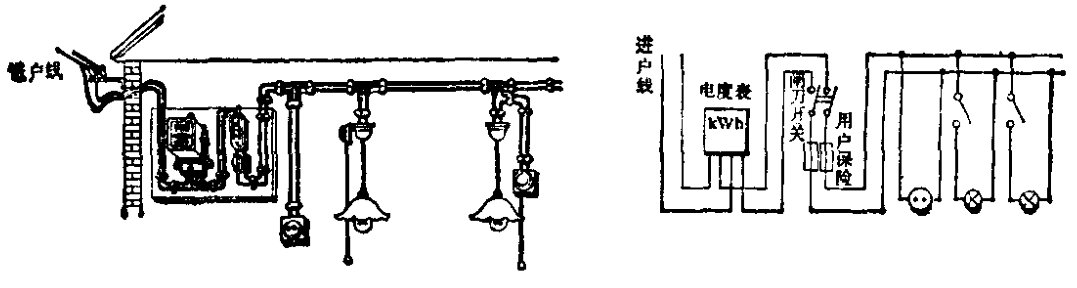
\includegraphics[width=\textwidth]{../pic/czwl2-ch11-1}
    \caption{室内照明电路的组成}\label{fig:11-1}
\end{figure}

